% ============================================================================
%  Chapter 3. Cohort Construction and Medication Extraction
%
%  \input file. No preamble. The parent document must load:
%      \usepackage{booktabs}   % \toprule \midrule \bottomrule \cmidrule
%      \usepackage{amsmath}    % aligned display math
%      \usepackage{graphicx}   % (only if figure assets are substituted in)
%      \usepackage[round]{natbib}  % \citep \citet
%  Bibliography: accord/thesis/refs.bib
%
%  Every quantity in this chapter is traceable to accord/phase1_cohort.py,
%  accord/phase2_medication.py, accord/dictionaries.py, or to the run logs
%  enumerated in accord/CORRECTIONS.md. Numbers with no such trace are marked
%  [TODO] rather than estimated.
% ============================================================================

\chapter{Cohort Construction and Medication Extraction}
\label{ch:data}

\section{What This Chapter Establishes}
\label{sec:data-overview}

This chapter builds the substrate that the rest of the thesis operates on: a set
of admissions in which a nursing progress note and a discharge summary both
exist, and a table of medication mentions extracted from those notes with an
action label attached to each. Everything downstream, the candidate rules of
Chapter~\ref{ch:candidates}, the weak labels of Chapter~\ref{ch:weak}, the model
of Chapter~\ref{ch:arch}, and the evaluation of Chapter~\ref{ch:eval}, consumes
this table and inherits its defects.

The chapter is written to make those defects legible in advance. Two of them
matter enough to state at the outset. First, \texttt{CHARTTIME} is null for
every discharge summary in MIMIC-III, which removes the ability to order a
discharge summary against anything else in time and, as
Section~\ref{sec:charttime} shows, silently converts several downstream
operations that look temporal into operations that are not. Second, the
extractor recovers roughly nine times as many action-classified medication
mentions from discharge summaries as from nursing notes, an asymmetry of
$79{,}385$ to $8{,}951$. Any pairwise rule defined over the two note types
therefore operates on two populations of radically different density, and the
rule yields reported in Chapter~\ref{ch:candidates} are shaped by that asymmetry
before any clinical content enters the picture.

Neither observation is a failure of the modelling that follows. Both are
properties of the data layer that the modelling had no way to overcome and,
in the original pipeline, no instrument to detect.

\section{Data Source, Access, and Handling}
\label{sec:source}

All experiments use MIMIC-III v1.4 \citep{johnson2016mimic}, a de-identified
critical-care database covering admissions to the Beth Israel Deaconess Medical
Center. The database is available only to credentialed users under a data use
agreement; access for this work was obtained through the standard PhysioNet
credentialing route.

Four tables are used: \texttt{ADMISSIONS} (admission and discharge timestamps,
demographics), \texttt{PATIENTS} (subject-level identifiers and dates of birth),
\texttt{DIAGNOSES\_ICD} (ICD-9 codes per admission), and \texttt{NOTEEVENTS}
(free-text clinical notes with a category label, a chart date, and, for some
categories, a chart time).

\paragraph{Text handling.} No clinical note text appears anywhere in this
thesis, in any figure, table, appendix, or supplementary artifact. All
note-derived text produced by the pipeline is written to a gitignored
\texttt{local\_only/} directory and never leaves the analysis machine. Reported
quantities are aggregate counts, rates, and model scores. Where a qualitative
observation is made about note content, it is stated abstractly rather than
quoted.

\paragraph{De-identification and its consequences.} MIMIC-III notes are
de-identified by an automated system that replaces protected health information
with bracketed surrogate tokens \citep{neamatullah2008deid}. This is not a
neutral transformation for our purposes. Surrogate tokens are dense at the head
of a note, where name, date, service, and identifier fields cluster.
Section~\ref{subsec:truncation-preview} notes the consequence, and
Chapter~\ref{ch:arch} develops it: a model that truncates a note to its first
$256$ WordPiece tokens is, for a substantial fraction of notes, reading a
de-identification header rather than a clinical narrative.

\section{Cohort Definition}
\label{sec:cohort}

\subsection{Index condition}

The primary cohort is heart failure, selected because polypharmacy is the norm
rather than the exception in this population and because the medications
involved, loop diuretics, beta blockers, anticoagulants, and antiarrhythmics,
have narrow therapeutic windows and well-documented harm profiles when
continued inappropriately. Admissions were selected by matching any ICD-9 code
against the prefix \texttt{428} in \texttt{DIAGNOSES\_ICD}.

Two secondary cohorts were constructed for the transfer experiments reported in
Chapter~\ref{ch:arch}: sepsis (ICD-9 prefix \texttt{038}) and acute kidney injury
(ICD-9 prefix \texttt{584}). These are prefix matches on billing codes and are
weaker cohort definitions than the physiologic criteria a clinical study would
use. They are adequate for the single purpose they serve here, which is to test
whether a model trained on heart failure retains any performance outside it.

\subsection{Filtering and yield}

Table~\ref{tab:cohort} reports the cohort at each filtering step. The only
clinical filter applied beyond the diagnosis code is $\mathrm{LOS} > 0$, which
removes admissions whose recorded discharge time precedes or equals their
admission time. These are data-entry artifacts rather than clinical events.

\begin{table}[t]
\centering
\small
\begin{tabular}{lrrr}
\toprule
 & \textbf{Heart failure} & \textbf{Sepsis} & \textbf{AKI} \\
 & (ICD-9 \texttt{428}) & (ICD-9 \texttt{038}) & (ICD-9 \texttt{584}) \\
\midrule
Admissions matching ICD-9 prefix & 13,608 & 6,265 & 11,422 \\
After $\mathrm{LOS} > 0$         & 13,597 & n/a   & n/a    \\
Unique patients                   & 10,143 & [TODO] & [TODO] \\
Median LOS (hours)                & 198.7  & [TODO] & [TODO] \\
\midrule
Admissions with a usable note pair & 9,783 & 4,339 & 7,579 \\
\bottomrule
\end{tabular}
\caption{Cohort construction. The heart-failure cohort is the training and
evaluation cohort; sepsis and AKI are used only for the transfer test in
Chapter~\ref{ch:arch}. The $\mathrm{LOS} > 0$ filter removes eleven
heart-failure admissions. The corresponding intermediate counts for the two
transfer cohorts were not preserved in the run logs and are marked [TODO]
rather than back-computed.}
\label{tab:cohort}
\end{table}

\paragraph{A defect in how this filter was applied.}
The reference implementation computes $\mathrm{LOS} > 0$ and reports the
resulting count of $13{,}597$, but assigns the result to a copy that is never
used again. Every downstream note join in the original pipeline runs against the
unfiltered $13{,}608$-admission set. The eleven-admission difference is
immaterial to any conclusion in this thesis. The defect is reported because it
is the first instance of a pattern that recurs at every stage: a quantity is
computed, printed, and treated as if it constrained the pipeline, while the code
path that would have applied it does not exist. The rebuilt
\texttt{accord/phase1\_cohort.py} applies the filter to the set that is actually
joined against, and the coverage percentages in
Section~\ref{sec:role-assignment} are reported against both denominators so that
the two are not confused.

\section{The Note-Role Assignment Problem}
\label{sec:role-assignment}

\subsection{The construct}

The clinical hypothesis motivating this thesis is that different clinical note
types carry different institutional weight. A nursing progress note recording
that a diuretic was withheld is a factual account of what happened at the
bedside. A discharge summary instructing that the same diuretic be continued at
a stated dose is an order that governs the patient's behaviour after they leave
the building. When these disagree, the disagreement is not symmetric: the
discharge summary is the document the patient and the receiving clinician will
act on, and the nursing note carries the information that would have made the
order wrong.

We refer to this construct as \emph{clinical note priority}. It is a property of
document type, not of individual authorship, and it is what
Chapter~\ref{ch:arch}'s authority conditioning mechanism was designed to
exploit. Chapter~\ref{ch:arch} also shows that the mechanism did not learn it.

\subsection{Six attempts at a three-role partition}

The original design used three roles: a nursing note, a discharge summary, and a
physician or admission note that would provide a third view of the medication
plan. Realising this partition against MIMIC-III's \texttt{CATEGORY} field
proved to be the single largest source of design change in the project. Six
configurations were attempted. Table~\ref{tab:roles} records the four for which
the definition and the resulting coverage survive in the run logs.

\begin{table}[t]
\centering
\small
\begin{tabular}{clr}
\toprule
\textbf{Attempt} & \textbf{Role definition} & \textbf{Coverage} \\
\midrule
1 & Three roles: nursing $+$ discharge $+$ physician                       & 16.7\% \\
2 & Three roles, broadened admission-note definition                       & 16.8\% \\
3 & Three roles, third role $=$ any non-radiology note within 24\,h of \texttt{ADMITTIME} & 12.4\% \\
4, 5 & [TODO: definitions not recoverable from surviving artifacts]        & [TODO] \\
6 & \textbf{Two roles: nursing $+$ discharge} (adopted)                    & \textbf{72.2\%} \\
\bottomrule
\end{tabular}
\caption{Note-role assignment attempts. Coverage is the fraction of
heart-failure admissions for which every required role is present, computed
against the $13{,}608$-admission ICD-9 set. Broadening the third role's
definition changed coverage by 0.1 percentage points (attempt 2); replacing it
with a purely temporal criterion made coverage worse (attempt 3). Dropping the
third role entirely raised coverage by more than a factor of four. Two
intermediate configurations are recorded in the project history without a
recoverable definition and are marked [TODO] rather than reconstructed.}
\label{tab:roles}
\end{table}

Two things in Table~\ref{tab:roles} deserve attention. Attempt 2 shows that the
three-role coverage ceiling is not an artifact of a narrow definition: relaxing
what counts as an admission note moved coverage by one tenth of a percentage
point. Attempt 3 shows that the ceiling is not an artifact of category naming
either, because a definition that ignores \texttt{CATEGORY} entirely and uses
only a time window performs worse. The limiting factor is that the physician
note types in MIMIC-III are unevenly populated across the covered period, and
requiring all three roles simultaneously intersects three sparse conditions.

\subsection{The retreat, and what it costs}

The adopted design drops the third role. This is a genuine loss and should be
recorded as such. With three roles the pipeline could have distinguished a
nursing/physician disagreement (a within-stay communication failure) from a
nursing/discharge disagreement (a failure that reaches the patient), and could
have used the physician note as an intermediate state against which to check
whether a conflict was resolved before discharge. With two roles neither is
possible. Section~\ref{sec:charttime} and Chapter~\ref{ch:candidates} show that
the attempt to recover the second capability by keyword matching produced an
instrument that did not measure what it claimed.

The two-role partition assigns \texttt{CATEGORY} values as follows:
\texttt{discharge summary} $\rightarrow$ \emph{discharge}; \texttt{nursing} and
\texttt{nursing/other} $\rightarrow$ \emph{nursing}; everything else discarded.
Under this partition $9{,}825$ of $13{,}608$ heart-failure admissions
($72.2\%$) have at least one note of each role.

\subsection{Note selection within an admission}

An admission may contain dozens of nursing notes and, in roughly one in seven
cases, more than one discharge-summary row (a Report and one or more Addenda).
One note per role per admission is selected:

\begin{itemize}
\item \textbf{Nursing note:} the note with the latest \texttt{CHARTTIME}
      strictly earlier than \texttt{DISCHTIME}. This is the last documented
      bedside state before the patient leaves, which is the state a discharge
      order should be consistent with.
\item \textbf{Discharge summary:} the first discharge-summary row
      chronologically.
\end{itemize}

Applying the nursing-selection constraint, which requires a non-null
\texttt{CHARTTIME} strictly before \texttt{DISCHTIME}, reduces the $9{,}825$
role-covered admissions to $9{,}783$ admissions for which both a nursing note
and a discharge summary can actually be selected. The final note table therefore
contains $9{,}783$ nursing rows and $9{,}783$ discharge rows, $19{,}566$ rows in
total.\footnote{An earlier project summary records this as ``$9{,}783$ nursing
$+$ $9{,}825$ discharge $=$ $19{,}566$ rows,'' which does not sum. The correct
statement is that $9{,}825$ admissions have both \emph{roles present} and
$9{,}783$ admissions survive \emph{note selection}; the paired table is
$2 \times 9{,}783$. The discrepancy is a documentation error, not a data error,
and is recorded here because the $9{,}825$ figure is quoted elsewhere in the
project as if it were the final cohort size.}

\section{The \texttt{CHARTTIME} Absence}
\label{sec:charttime}

\subsection{The finding}

\texttt{CHARTTIME} is null for $100\%$ of discharge-summary rows in MIMIC-III.
Discharge summaries are written retrospectively, often after the patient has
left, and the database records only a \texttt{CHARTDATE}. This is a documented
property of the resource rather than a corruption, but it has consequences that
were not recognised in the original pipeline.

\subsection{Consequence 1: ``first discharge summary'' was not chronological}

The reference implementation selects the discharge summary with
\texttt{groupby('HADM\_ID').first()} applied to an unsorted frame. Read
casually, this is ``the first note charted.'' Because \texttt{CHARTTIME} is
null, it is in fact ``whichever row happened to appear first in the
concatenation order of the chunked read,'' which is a function of file layout
and chunk size. $14.8\%$ of the final $9{,}783$ admissions ($1{,}448$) have more than one
discharge-summary row, so this is not a corner case: for about one admission in
seven, the note the pipeline treated as the governing discharge order was
selected arbitrarily between a Report and its Addendum.

The rebuilt implementation sorts on \texttt{CHARTDATE}, the field that
\emph{is} populated for discharge summaries, with \texttt{ROW\_ID} as a
deterministic tie-break, before taking the first row. This restores determinism.
It does not restore chronology at sub-day resolution, which the data does not
contain.

\subsection{Consequence 2: no temporal ordering between the paired notes}

Because the nursing note has a timestamp and the discharge summary has only a
date, the pipeline cannot in general establish that the nursing note precedes
the discharge summary at anything finer than day granularity, and cannot
establish an ordering at all between a discharge summary and any other
same-day note. Every claim in this thesis that depends on ``the nursing note
came first'' rests on the selection rule (last nursing note strictly before
\texttt{DISCHTIME}) rather than on a measured comparison against the discharge
summary's timestamp, because no such timestamp exists.

\subsection{Consequence 3: an intermediate-documentation filter that could not work}

A natural objection to any cross-note contradiction detector is that the
apparent conflict may have been resolved by documentation written between the
two notes. The original pipeline attempted to quantify this with a keyword
filter over intervening text and reported that only $2$ of $1{,}610$ filterable
candidates were resolved by intermediate documentation, presenting this as
evidence for the clinical need the system addresses.

This claim is withdrawn. Three earlier versions of the filter returned zero
resolved candidates for the direct reason that \texttt{CHARTTIME} is null for
every discharge summary, so the interval within which to search was empty. The
version that returned a non-zero count used a resolution pattern that is a
twenty-way alternation containing both directions of the medication decision
simultaneously (\texttt{resume}, \texttt{restart}, \texttt{continue}, and in the
same alternation \texttt{discontinue}, \texttt{hold}, \texttt{stop}). It matches
nearly any sentence about a medication, and a match anywhere within $\pm 2$
lines was counted as a resolution. A filter that matches almost everything and
returns two positives out of $1{,}610$ is reporting the behaviour of its own
search window, not the behaviour of clinicians. The correct statement is the
one this section makes: the temporal information required to test the
intermediate-documentation hypothesis is absent from the resource, so the
hypothesis remains untested.

\section{Medication Mention Extraction}
\label{sec:extraction}

\subsection{Why a dictionary extractor}

Clinical medication extraction is a mature task with strong published systems
\citep{uzuner2010medication,henry2020n2c2} and mature tooling
\citep{neumann2019scispacy,eyre2021medspacy}. This project used neither.

Installation of scispaCy and medspaCy was attempted and abandoned: dependency
resolution against the pinned spaCy version in the analysis environment failed
repeatedly, and rather than resolve it the project proceeded with a dictionary
extractor over spaCy's \texttt{en\_core\_web\_sm} pipeline. This is a
methodological weakness and is stated plainly rather than presented as a design
choice. Its most likely effect is a systematic loss of recall on drug names
outside the seed dictionary, on inflected and misspelled forms, and on
multi-token brand names, and a systematic loss of precision on negation and
scope, where a purpose-built ConText or NegEx implementation
\citep{chapman2001negex} would outperform the regular-expression alternation
used here.

\subsection{Dictionaries}

The extractor is built on four hand-written resources, reproduced verbatim in
\texttt{accord/dictionaries.py}:

\begin{enumerate}
\item \textbf{\texttt{HF\_DRUGS}}: 77 heart-failure-relevant generic drug
      names.\footnote{A recount of the committed dictionary enumerates 77
      string literals. The figure 76 appears in the original run log. The
      discrepancy is one entry and is [TODO: reconcile against the exact
      dictionary state at the time of the production run]. It does not affect
      any reported count, since all extraction counts are measured rather than
      derived from the dictionary size.}
\item \textbf{\texttt{ABBREV}}: 21 abbreviation and brand-name expansions
      (\texttt{lasix} $\rightarrow$ \texttt{furosemide}, \texttt{coreg}
      $\rightarrow$ \texttt{carvedilol}, and so on).
\item \textbf{\texttt{VARIANTS}}: 6 spelling and formulation normalisations
      (\texttt{metoprolol succinate} and \texttt{metoprolol tartrate} both
      $\rightarrow$ \texttt{metoprolol}).
\item \textbf{\texttt{ACTION\_PATTERNS}}: four regular-expression alternations
      defining the action classes \emph{cessation}, \emph{continuation},
      \emph{initiation}, and \emph{dose modification}, plus a separate
      \texttt{NEGATION} alternation.
\end{enumerate}

The union of these sources is 105 matchable strings collapsing to 79 distinct normalised targets. Matching is
case-insensitive with regular-expression word boundaries on both sides, applied after
abbreviation and variant expansion of the note text.

\subsection{Action classification}

For each sentence, a context window comprising the previous, current, and next
sentence is assembled. The \texttt{NEGATION} pattern is applied to that window
to produce a boolean. The four \texttt{ACTION\_PATTERNS} are then applied to the
same window in a fixed order (\emph{cessation}, \emph{continuation},
\emph{initiation}, \emph{dose modification}), and the \emph{first} pattern that
matches determines the raw action; if none matches the mention is
\emph{unclassified}. Negation then rewrites the raw action:

\begin{center}
\begin{tabular}{ll}
\toprule
\textbf{Raw action, negated} & \textbf{Final action} \\
\midrule
continuation & cessation \\
initiation   & cessation \\
cessation    & continuation \\
\bottomrule
\end{tabular}
\end{center}

\paragraph{Three properties of this design that shape everything downstream.}
First, the action is a property of a three-sentence \emph{window}, not of the
drug mention, so every drug mentioned anywhere in that window receives the same
action label. A sentence listing five medications after a sentence containing
``held'' assigns \emph{cessation} to all five. Second, first-match ordering
makes the classes non-exclusive in effect: a window containing both ``held'' and
``continue'' resolves to \emph{cessation} because \emph{cessation} is tested
first. Third, the negation rewrite is a hard flip with no scope model, so a
window containing \emph{cessation} vocabulary and any negation cue anywhere
within it becomes \emph{continuation}. Chapter~\ref{ch:candidates} shows that
Rules 1 and 2 are defined entirely over these action labels, which means the
candidate pool inherits all three properties directly.

\subsection{Dose parsing}

The reference extractor stored the raw matched dose string and discarded
offsets. The rebuild adds a numeric parser that reduces a dose to a
\texttt{(value, canonical\_unit)} pair, converting within the mass family
(\texttt{mcg}, \texttt{mg}, \texttt{g} $\rightarrow$ \texttt{mg}) and keeping
\texttt{mEq}, \texttt{unit}, and \texttt{ml} as separate incomparable units,
since converting them requires drug-specific molar mass or dilution information
the resource does not provide. Two doses are compared only when their canonical
units match. This parser did not exist in the reference implementation, which is
why the dosage rule of Chapter~\ref{ch:candidates} has no source code in the
original pipeline: without a numeric value there is nothing from which to
compute a percentage difference.

\subsection{Offsets, and why their absence mattered}

The rebuild additionally records, for every mention, its sentence index within
the note and character offsets for the sentence span, the drug match, and the
dose match. The reference implementation recorded none of these. This is not a
convenience difference. It is the direct enabling condition of the most
consequential defect in the pipeline: with no positional information in the
mentions table, nothing downstream could distinguish one mention of a drug from
another mention of the same drug in the same note, which is precisely what the
candidate-mining code needed to do and did not.
Chapter~\ref{ch:candidates} measures the cost.

\section{Extraction Yield}
\label{sec:yield}

\begin{table}[t]
\centering
\small
\begin{tabular}{lr}
\toprule
\textbf{Quantity} & \textbf{Value} \\
\midrule
Notes processed & 19,566 \\
Total medication mentions & 219,683 \\
Mentions with a resolved action & 88,336 \\
\quad of which, from discharge summaries & 79,385 \\
\quad of which, from nursing notes & 8,951 \\
Mentions unclassified & 131,347 \\
Unique normalised drugs observed & 70 \\
Admissions with at least one mention & 9,732 \\
\bottomrule
\end{tabular}
\caption{Medication extraction yield over the heart-failure note pairs. Note the
denominator: only $40.2\%$ of mentions receive an action label at all, and among
those that do, discharge summaries contribute $89.9\%$. The $70$ unique drugs
observed against a seed dictionary of roughly $90$ matchable strings indicates
that a fifth of the dictionary never fired.}
\label{tab:yield}
\end{table}

\subsection{The nursing/discharge asymmetry}

Table~\ref{tab:yield} contains the most important number in this chapter.
Discharge summaries yield $79{,}385$ action-classified mentions; nursing notes
yield $8{,}951$. The ratio is $8.9$ to $1$, from an equal number of notes on
each side.

The asymmetry has an obvious proximate explanation. A discharge summary contains
an explicit, structured medication list, often with an accompanying narrative of
medication changes, and it is written to be a complete account. A nursing
progress note is a shift-scoped narrative that mentions a medication only when
something about it is worth recording. The asymmetry is therefore real clinical
structure, not an extraction artifact alone. But its consequence for this
pipeline is severe and was not accounted for in the original design:

\begin{itemize}
\item Every rule in Chapter~\ref{ch:candidates} that requires a matching drug on
      both sides is bottlenecked by the nursing side. The effective universe for
      a paired rule is roughly $8{,}951$ mentions, not $88{,}336$.
\item The omission rule (drug held in nursing, absent from discharge) runs
      against the \emph{dense} side, so its absence condition is comparatively
      well-evidenced. Rules 1 through 3 run against the sparse side, so their
      presence condition is comparatively poorly evidenced.
\item Any model that consumes a nursing sentence and a discharge sentence is
      being given, on average, a much more informative discharge input. A model
      that learned to ignore the nursing input entirely would lose little
      signal. Chapter~\ref{ch:arch} shows a model that appears to have done
      something close to this, and Chapter~\ref{ch:eval} shows that its
      predictions do not depend on the pair in any measurable way.
\end{itemize}

\subsection{The unclassified majority}

Nearly $60\%$ of mentions receive no action label. This is the expected
behaviour of a closed pattern set applied to open text: the four action
alternations cover an explicit decision vocabulary, and most medication mentions
in clinical narrative are not explicit decisions. They are list entries,
allergy-section references, historical mentions, or problem-list context.
Discarding them is defensible. The relevant consequence is that the classified
subset is not a random sample of mentions; it is enriched for sentences
containing decision vocabulary, which is exactly the population in which the
first-match ordering and negation-flip defects of
Section~\ref{sec:extraction} are most likely to fire.

\subsection{Truncation and the de-identification header}
\label{subsec:truncation-preview}

One observation recorded here for use in Chapter~\ref{ch:arch}: the model
described there truncates each note to its first $256$ WordPiece tokens, taken
from the head of the note. In MIMIC-III discharge summaries the head of the note
is the administrative header block, which is where the de-identification
surrogates are densest. A $256$-token head-truncation of a discharge summary
frequently contains no medication content at all. This is a property of the data
representation interacting with a modelling choice, and it is one of the two
visible mechanisms behind the pretraining collapse documented in
Section~\ref{sec:stage0}.

\section{Proposed Figures}
\label{sec:data-figures}

\begin{figure}[t]
\centering
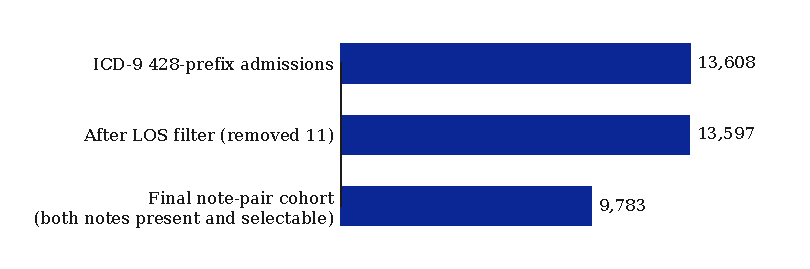
\includegraphics[width=0.92\linewidth]{figures/fig-funnel.pdf}
\caption{Cohort funnel. The reader should notice that the single largest design
decision in the data layer, dropping the third note role, is worth more than a
factor of four in coverage, and that no refinement of the three-role definition
recovered it.}
\label{fig:funnel}
\end{figure}

\begin{figure}[t]
\centering
\framebox[\linewidth]{\parbox[c][5cm][c]{0.92\linewidth}{\centering
\textit{[Figure asset 3.2: two-panel. Left, stacked bar of the 219,683 mentions}
\textit{split classified (88,336) / unclassified (131,347). Right, the 88,336}
\textit{classified mentions split by note role, 79,385 discharge vs 8,951}
\textit{nursing, drawn to scale so the 8.9:1 ratio is visually unavoidable.]}}}
\caption{Extraction yield and the note-role asymmetry. The right panel is the
constraint that governs Chapter~\ref{ch:candidates}: every paired rule is
limited by the smaller population, and every model that consumes a note pair
receives systematically unequal evidence from its two inputs.}
\label{fig:asymmetry}
\end{figure}

\section{Limitations of the Data Layer}
\label{sec:data-limitations}

The following are limitations of this chapter's output, independent of anything
that happens downstream.

\paragraph{Single institution, single era, critical care only.} MIMIC-III covers
one academic medical centre. Documentation conventions, note-type taxonomies,
and medication-list formatting are institution-specific. Nothing in this chapter
transfers without re-derivation.

\paragraph{Billing codes are not clinical phenotypes.} An ICD-9 prefix match
identifies admissions that were \emph{coded} for heart failure. It over-includes
admissions where heart failure is a comorbidity rather than the reason for
admission, and under-includes admissions where it was clinically present but
not coded. The sepsis and AKI cohorts are weaker still.

\paragraph{The extractor is a dictionary, not a clinical NER system.} Recall on
drugs outside the seed list is zero by construction. Negation is a
regular-expression alternation with no scope, and action classification is
window-scoped and first-match. Published clinical medication extraction systems
would be materially better on all three axes \citep{henry2020n2c2}, and the
decision not to use one was driven by an environment problem, not by evidence.

\paragraph{No annotation of the extraction itself.} The extractor's precision
and recall against a human-annotated mention set were never measured. Every
error rate reported later in this thesis is therefore an error rate of the
\emph{composed} system, and the contribution of extraction error to it cannot
be separated from the contribution of candidate-generation error or model error.
This is the most consequential missing measurement in the data layer. A
[TODO: annotate a sample of $n \approx 200$ sentences for drug mention and
action label, and report extractor precision/recall/$F_1$] would resolve it, and
should be the first item of any continuation of this work.

\paragraph{No temporal ordering at sub-day resolution.} Section~\ref{sec:charttime}.

\paragraph{The paired-note design discards within-stay evolution.} One nursing
note per admission, selected as the last one, discards every earlier nursing
note. A medication decision documented at hour 12 and reversed at hour 60 is
invisible; only the hour-60 state enters the pipeline. This is a deliberate
simplification that trades recall of within-stay conflict for tractability, and
it was never revisited.

\section{Ethical Considerations for the Data Layer}
\label{sec:data-ethics}

MIMIC-III is credentialed data governed by a data use agreement. The compliance
posture of this work is stated here in full, including where it is imperfect.

\paragraph{Note text.} No clinical note text appears in this document, in any
figure, table or appendix, or in any released artifact. Files containing
note-derived text are confined to a gitignored local directory outside the
version-controlled tree, and the export script that publishes results scans every
file for note-text markers and aborts rather than filtering on a hit. Released
artifacts are aggregate counts, rates, model scores and pair-level labels.

\paragraph{Third-party services.} The weak labeller in Chapter~\ref{ch:weak} is
an open-weights model run locally; no note text left the analysis machine for
that stage. The GPT-4o comparison reported in Chapter~\ref{ch:eval} was run
against a hosted commercial API, and note excerpts were transmitted to that API
as part of the prompt. Guidance issued during this project's lifetime identifies
transmission of credentialed data to general-purpose hosted APIs as inconsistent
with the data use agreement, and specifies compliant alternatives with
zero-retention and no-human-review terms. The GPT-4o rows are reported with that
caveat attached, and are retained because removing them would misrepresent the
comparison actually performed. No further transmission to hosted services has
occurred and none will occur in follow-on work.

\paragraph{Re-identification and disaggregation.} No re-identification was
attempted and no auxiliary dataset was joined against MIMIC-III at the patient
level. Subgroup analyses are reported as one-way marginals only; no multi-way
disaggregation is published. Cells below approximately ten observations are
reported without suppression, because the source data is de-identified under
HIPAA Safe Harbor and no identifier crosswalk is released. Such cells are
reported for transparency and are not powered to support inference; every claim
resting on them is qualified accordingly in Chapter~\ref{ch:eval}.

\paragraph{Clinical status.} Nothing in this work has been validated for
clinical use. The system is a research artifact evaluated on retrospective
de-identified data, it is not a clinical decision support tool, and its measured
performance --- reported in Chapter~\ref{ch:eval} --- does not support deployment
in any care setting.

\section{Summary}
\label{sec:data-summary}

This chapter produced $19{,}566$ note rows over $9{,}783$ heart-failure
admissions, and $88{,}336$ action-classified medication mentions over $9{,}732$
of them. It also produced four constraints that the rest of the thesis operates
under and cannot escape:

\begin{enumerate}
\item \textbf{The three-role design was abandoned}, at a coverage ceiling of
      $16.8\%$, in favour of a two-role design at $72.2\%$. The cost is that no
      intermediate document exists against which to check whether a conflict was
      resolved before discharge.
\item \textbf{\texttt{CHARTTIME} is null for every discharge summary}, which
      removes sub-day temporal ordering and invalidated a filter that had been
      reported as a clinical finding.
\item \textbf{Action-classified mentions are asymmetric by a factor of $8.9$}
      between discharge summaries and nursing notes, which bottlenecks every
      paired rule and gives every downstream model systematically unequal
      evidence from its two inputs.
\item \textbf{The extractor was never validated}, so no downstream error rate
      can be decomposed into extraction error and model error.
\end{enumerate}

Chapter~\ref{ch:candidates} builds four rules on top of this table and shows
that the mechanism which selects the evidence sentence for each candidate was
wrong for $41.4\%$ of action-conflict candidates.
